\section{Ejercicio 3}
En esta sección del presente informe se realizará la implementación fisica de la máquina de Moore que se puede ver en la figura \ref{ej3_diagrama_de_estados}.\\
Para ello se trabajará con entradas de señales de 5V y con lógica interna trabajando con tensiones de 3.3V.
\begin{figure}[H]
    \centering
    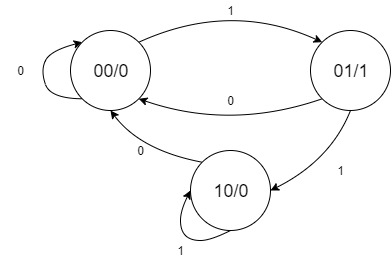
\includegraphics[width=0.6\textwidth]{figs/Ej3/FSM.jpg} % first figure itself
    \caption{Diagrama de estados de Moore a realizar.}
    \label{ej3_diagrama_de_estados}
\end{figure}
%
Así la tabla de estados correspondiente a la situación planteada se puede ver en la tabla \ref{ej3_table1}.
\begin{table}[H]
\caption{Tabla de Estados.}
\label{ej3_table1}
\centering
\begin{tabular}{|c|c|c|c|}
\hline
Estado actual         & \multicolumn{2}{c|}{Estado Siguiente} & Salida             \\ \hline
\multirow{2}{*}{y1y2} & I=0               & I=1               & \multirow{2}{*}{Z} \\ \cline{2-3}
                      & Y2Y1              & Y2Y1              &                    \\ \hline
00                    & 00                & 01                & 0                  \\ \hline
01                    & 00                & 10                & 1                  \\ \hline
10                    & 00                & 10                & 0                  \\ \hline
11                    & XX                & XX                & X                  \\ \hline
\end{tabular}
\end{table}
%
De esta manera los diagramas de Karnaugh del sistema quedan de la siguiente forma, tomando como ABC a y2, y1, I respectivamente.\\
%
Y1:
%
\begin{center}
    \begin{Karnaughvuit}
       \minterms{4}
        \maxterms{0,1,2,5,6}
        \indeterminats{3,7}
       \implicantsol{4}{red}
    \end{Karnaughvuit}
\end{center}
%
Y2:
%
\begin{center}
    \begin{Karnaughvuit}
       \minterms{5,6}
        \maxterms{0,1,2,4}
        \indeterminats{3,7}
       \implicant{5}{7}{green}
        \implicant{7}{6}{blue}
    \end{Karnaughvuit}
\end{center}
%
Z:
%
\begin{center}
    \begin{Karnaughquatre}
       \minterms{2}
        \maxterms{0,1}
        \indeterminats{3}
        \implicant{2}{3}{purple}
    \end{Karnaughquatre}
\end{center}
%
Así, las ecuaciones que se ajustan a los karnaught mostados se pueden ver en las ecuaciones \ref{ej3_eq}.
%
\begin{equation}
\begin{split}
    Y1&=I \cdot \overline{y1} \cdot \overline{y2}\\
    Y2&=y1 \cdot I+y2 \cdot I = (y1 + y2) I\\
    Z&=y1
\label{ej3_eq}
\end{split}
\end{equation}
%
De esta manera el circuito que cumple con estas ecuaciones se puede ver en la figura \ref{ej3_circuito}, en el mismo se decidió por utilizar solo compuertas nand y nor para evitar el uso excesivo de integrados. Ademas se destaca que para el pasaje de 5V a 3.3V se utilizó un diodo zener de 3.3V y una resistencia y para el pasaje de 5V a 3V se utilizó el circuito de la figura \ref{ej3_fig_5v}.
%
\begin{figure}[H]
    \centering
    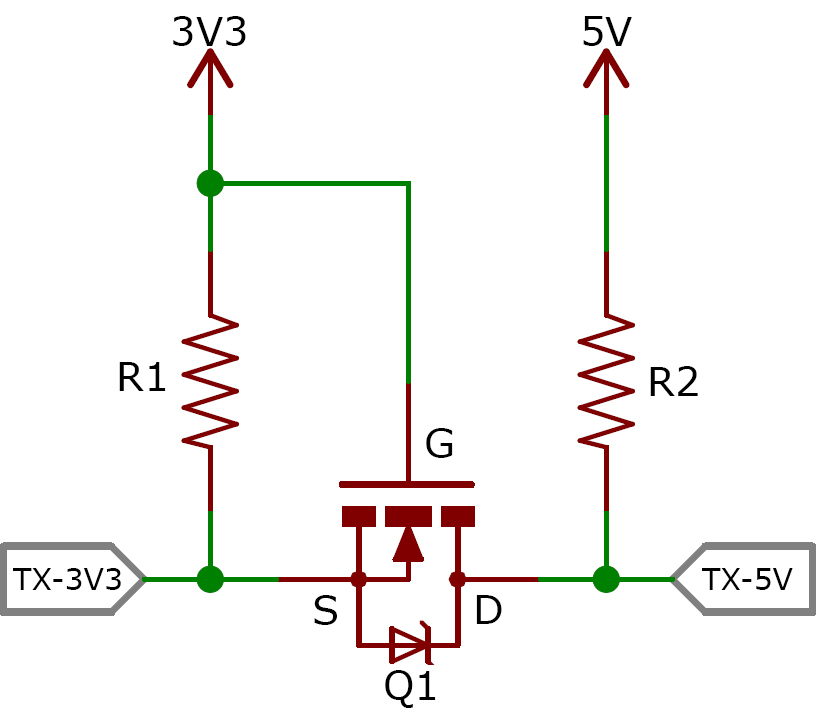
\includegraphics[width=0.3\textwidth]{figs/Ej3/shifter.JPG} % first figure itself
        \caption{Esquema del circuito para convertir 3.3V en 5V}
    \label{ej3_fig_5v}
\end{figure}
%
%
\begin{figure}[H]
    \centering
    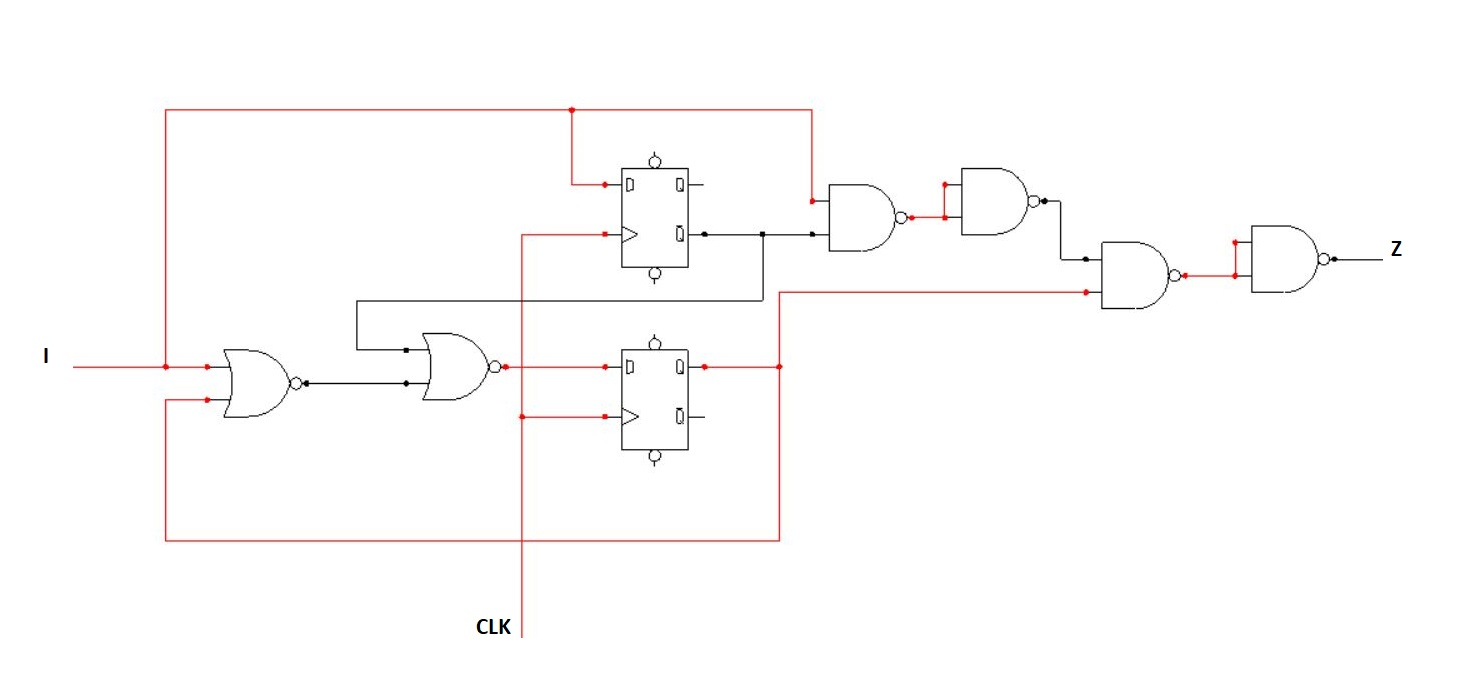
\includegraphics[width=1\textwidth]{figs/Ej3/circ_ej3.JPG} % first figure itself
        \caption{Esquemático del circuito a realizar.}
    \label{ej3_circuito}
\end{figure}
%
De esta manera se implementó el circuito en una placa PCB y se procedió a medir los resultados obtenidos, los mismos se pueden ver en las imagenes \ref{ej3_res1} y \ref{ej3_res2}.
%
\begin{figure}[H]
    \centering
    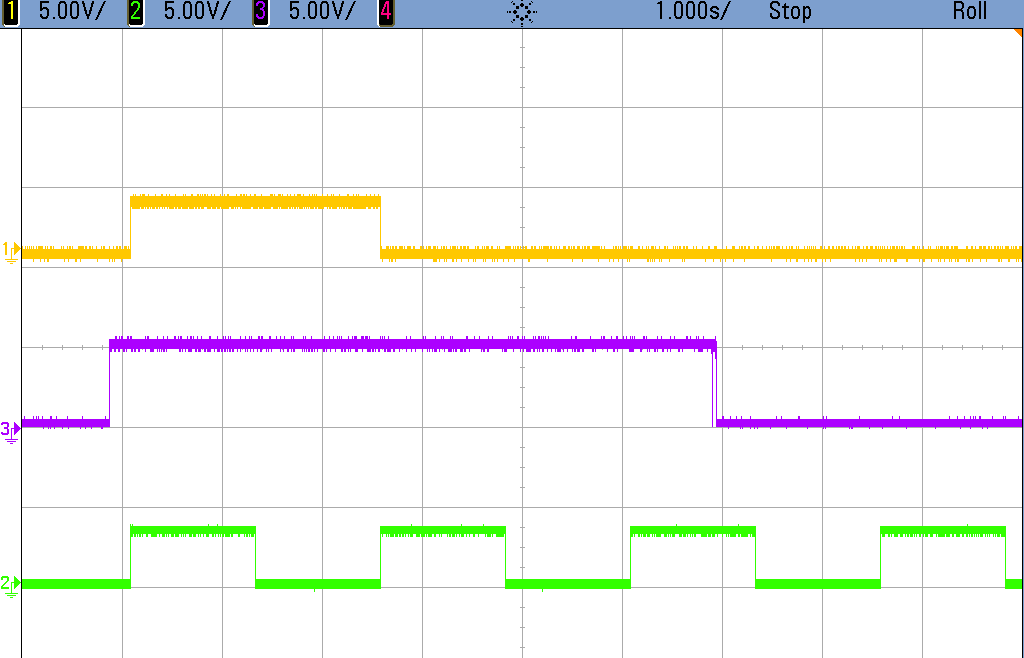
\includegraphics[width=0.6\textwidth]{figs/Ej3/scope_19.png} % first figure itself
        \caption{Respuesta del circuito al entrar con un 1 por mas de un tiempo de clock}
    \label{ej3_res1}
\end{figure}
%
%
\begin{figure}[H]
    \centering
    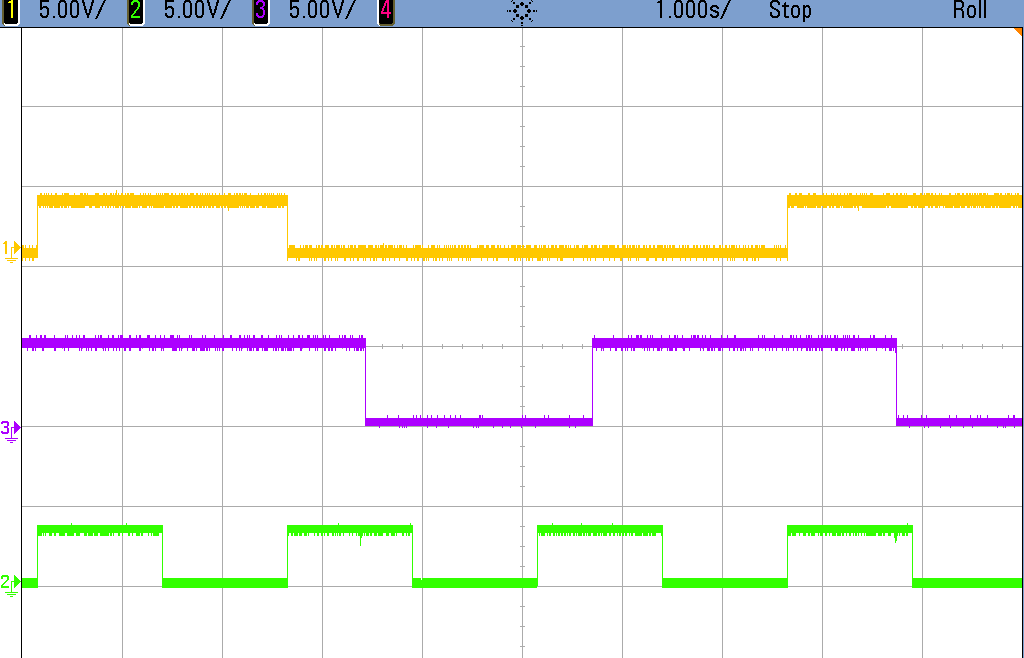
\includegraphics[width=0.6\textwidth]{figs/Ej3/scope_20.png} % first figure itself
        \caption{Respuesta del circuito al entrar dos veces con un uno}
    \label{ej3_res2}
\end{figure}
%
Se puede concluir a partir de las mediciones realizadas que el circuito funciona correctamente y por lo tanto el circuito se comporta como era esperado.